\documentclass{article}
\usepackage[utf8]{inputenc}
\usepackage{hyperref}
\usepackage[letterpaper, portrait, margin=1in]{geometry}
\usepackage{enumitem}
\usepackage{amsmath}
\usepackage{booktabs}
\usepackage{graphicx}

\usepackage{titlesec}

\titleformat{\section}
{\normalfont\Large\bfseries}{\thesection}{1em}{}[{\titlerule[0.8pt]}]
  
\title{Homework 6}
\author{Economics 7103}
  
\begin{document}
  
\maketitle

\section{Hourly data - Stata}
\noindent 1. I generated a treatment cohort variable and the number of treated cohorts is 539.

\noindent 2. The number of negative weights is  48,547.

\noindent 3. The TWFE regression results on hourly data are presented in the Table \ref{tab:TWFE}. I clustered on ID level because the function 'reghdfe' allows to obtain multi-way clustered standard errors, so we can account for multiple dimensions of clustering. 

\begin{table}[h]
    \centering
    \begin{tabular}{lc} \hline
 & (1) \\
VARIABLES & TWFE regression results on hourly data \\ \hline
 &  \\
Treatment & -0.0434*** \\
 & (0.000232) \\
Temperature (F) & 0.00461*** \\
 & (1.21e-05) \\
Precipitation (in) & -0.000644 \\
 & (0.00200) \\
Relative Humidity (\%) & 0.00230*** \\
 & (5.76e-06) \\
Constant & 0.539*** \\
 & (0.00111) \\
 &  \\
Observations & 720,000 \\
 R-squared & 0.664 \\ \hline
\multicolumn{2}{c}{ Robust standard errors in parentheses} \\
\multicolumn{2}{c}{ *** p$<$0.01, ** p$<$0.05, * p$<$0.1} \\
\end{tabular}

    \caption{TWFE Regression Results on Hourly Data}
    \label{tab:TWFE}
\end{table}

\clearpage

\section{Daily data - Stata}

\noindent 1. The TWFE regression results on daily data are presented in the Table \ref{tab:TWFEdaily}. We need to transform the coefficient obtained from hourly data to make it comparable with the daily coefficient. $-0.0434 * 24 = -1.1856$, which is higher than the coefficient from daily energy consumption data. This might be caused by losing hourly trends of energy consumption in the daily dataset. 


\begin{table}[h]
    \centering
    \begin{tabular}{lc} \hline
 & (1) \\
VARIABLES & TWFE (Daily) \\ \hline
 &  \\
Treatment & -0.936*** \\
 & (0.00557) \\
Temperature (F) & 0.111*** \\
 & (0.000379) \\
Precipitation (in) & 0.0681 \\
 & (0.188) \\
Relative Humidity (\%) & 0.0552*** \\
 & (0.000189) \\
Constant & 12.88*** \\
 & (0.0341) \\
 &  \\
Observations & 30,000 \\
 R-squared & 0.972 \\ \hline
\multicolumn{2}{c}{ Robust standard errors in parentheses} \\
\multicolumn{2}{c}{ *** p$<$0.01, ** p$<$0.05, * p$<$0.1} \\
\end{tabular}

    \caption{TWFE Regression Results on Hourly Data}
    \label{tab:TWFEdaily}
\end{table}

\clearpage

\noindent 2. \textbf{NOTE: }I used Afi's code for this section. I tried to plot event study using 'coefplot' as you suggested but the graph was very unclear. I will come back to this function again to understand. 

The event study is presented on the Figure \ref{fig:eventstudy1}

\begin{figure}
    \centering
    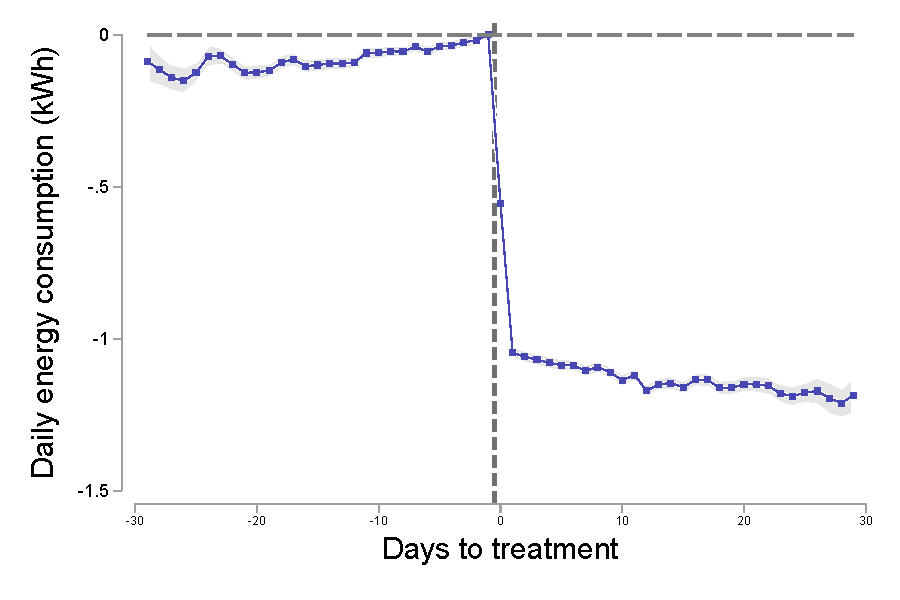
\includegraphics{homework 6/output/figure/event_study.pdf}
    \caption{Event Study  Using 'reghdfe'}
    \label{fig:eventstudy1}
\end{figure}


\clearpage

\noindent 3. The event study using the command "eventdd" is presented on the Figure \ref{fig:eventstudy2}

\begin{figure}
    \centering
    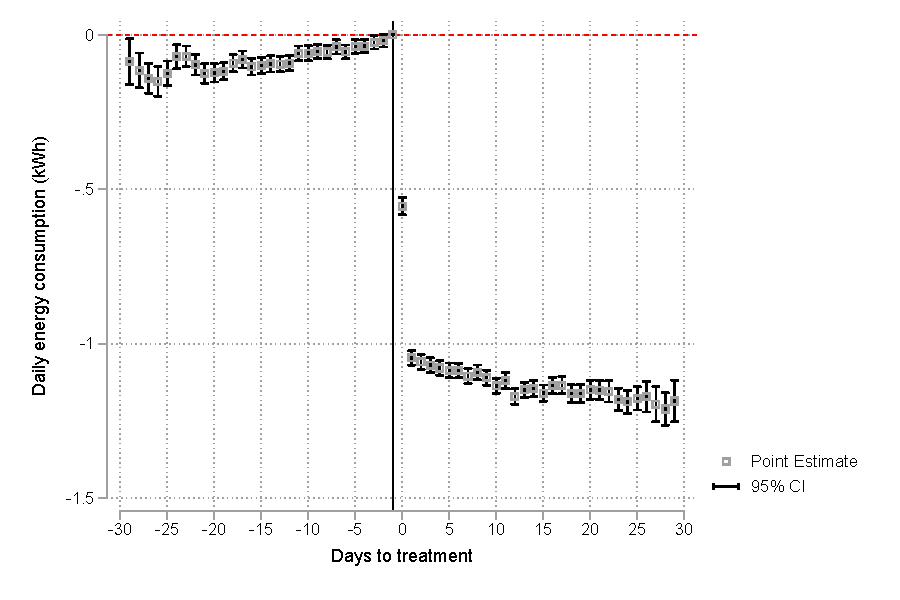
\includegraphics{homework 6/output/figure/event_study_1.pdf}
    \caption{Event Study  Using 'eventdd'}
    \label{fig:eventstudy2}
\end{figure}

\noindent 4.The event study using the command "ecsdid" is presented on the Figure \ref{fig:eventstudy3}

\begin{figure}
    \centering
    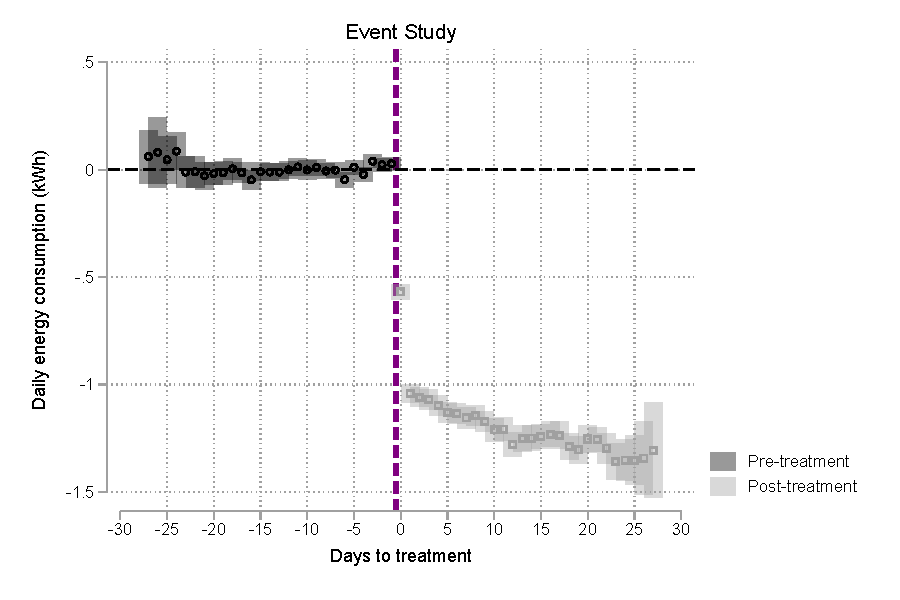
\includegraphics{homework 6/output/figure/event_study_csdid.pdf}
    \caption{Event Study  Using 'csdid'}
    \label{fig:eventstudy3}
\end{figure}

\end{document}